如图是某校学生上学方式的统计情况,则下列说法正确的是\key{}
\fourchoices{水平的数轴表示的含义是人数}{竖直的数轴表示的含义是来校方式}{乘私家车来校的学生人数最多}{骑自行车来校的学生人数最少}
\begin{center}
    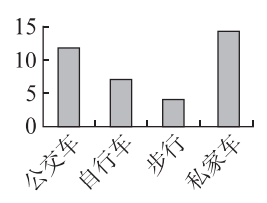
\includegraphics[height=6cm]{lib/image/MJA03050202.png}
\end{center}